%# -*- coding: utf-8-unix -*-
%%==================================================
%% thesis.tex
%%==================================================

% 双面打印
\documentclass[bachelor, openright, twoside, english]{sjtuthesis}
% \documentclass[bachelor, openany, oneside, submit]{sjtuthesis}
% \documentclass[master, review]{sjtuthesis}
% \documentclass[%
%   bachelor|master|doctor,	% 必选项
%   fontset=fandol|windows|mac|ubuntu|adobe|founder, % 字体选项
%   oneside|twoside,		% 单面打印,双面打印(奇偶页交换页边距,默认)
%   openany|openright, 		% 可以在奇数或者偶数页开新章|只在奇数页开新章(默认)
%   english,			% 启用英文模版
%   review,	 		% 盲审论文,隐去作者姓名、学号、导师姓名、致谢、发表论文和参与的项目
%   submit			% 定稿提交的论文,插入签名扫描版的原创性声明、授权声明 
% ]

% 逐个导入参考文献数据库
\addbibresource{bib/thesis.bib}
% \addbibresource{bib/chap2.bib}

\begin{document}

%% 无编号内容:中英文论文封面、授权页
%# -*- coding: utf-8-unix -*-
\title{基于机器教学的智能在线评测系统}
\author{陈乐群}
\advisor{俞勇教授}
% \coadvisor{某某教授}
\defenddate{2018年6月15日}
\school{上海交通大学}
\institute{致远学院}
\studentnumber{5140309565}
\major{计算机科学与技术(致远荣誉计划)}

\englishtitle{An Intelligent Online Judge System with Machine Teaching Techniques}
\englishauthor{\textsc{Lequn Chen}}
\englishadvisor{Prof. \textsc{Yong Yu}}
% \englishcoadvisor{Prof. \textsc{Uom Uom}}
\englishschool{Shanghai Jiao Tong University}
\englishinstitute{\textsc{Zhiyuan College} \\
  \textsc{Shanghai Jiao Tong University} \\
  \textsc{Shanghai, P.R.China}}
\englishmajor{Computer Science and Technology (Zhiyuan Honors Program)}
\englishdate{June 15th, 2018}


\maketitle

\makeatletter
\ifsjtu@submit\relax
	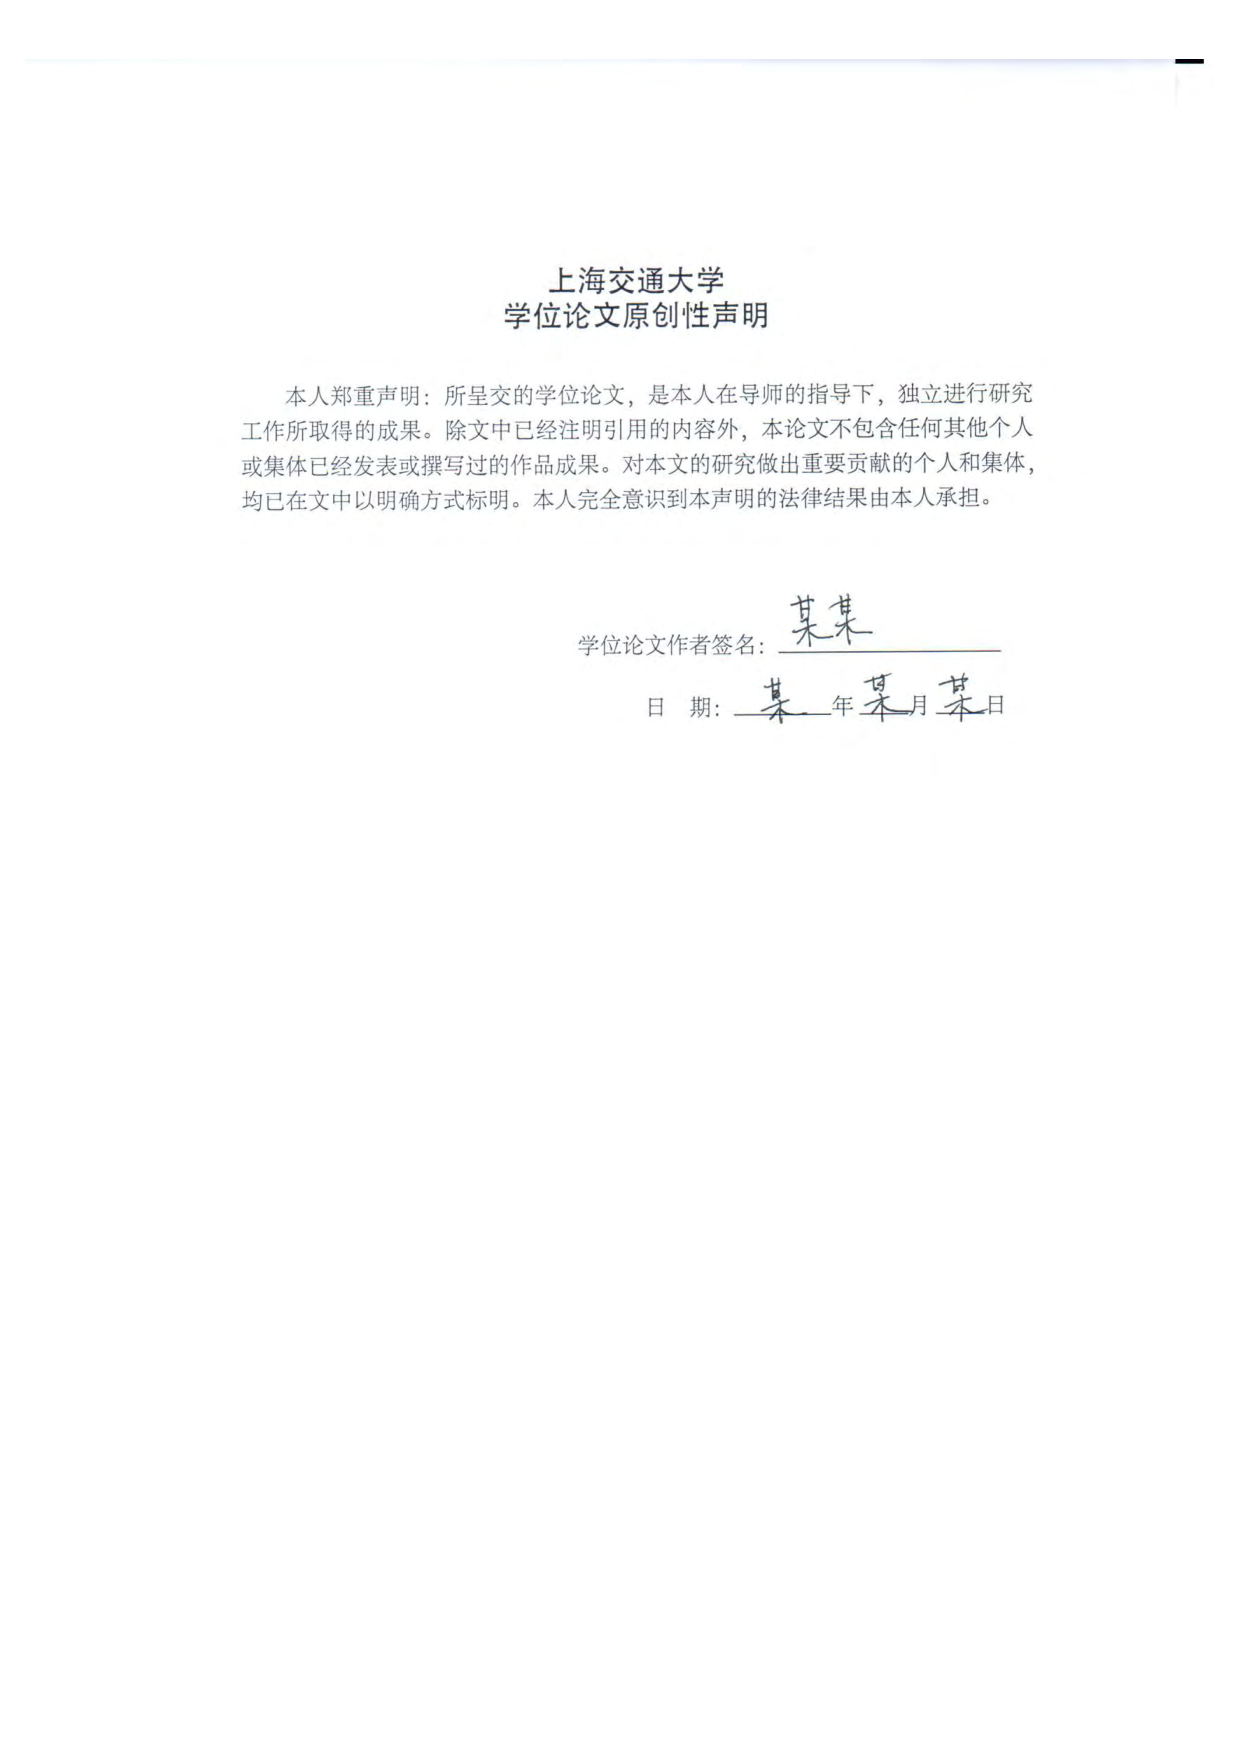
\includepdf{pdf/original.pdf}
	\cleardoublepage
	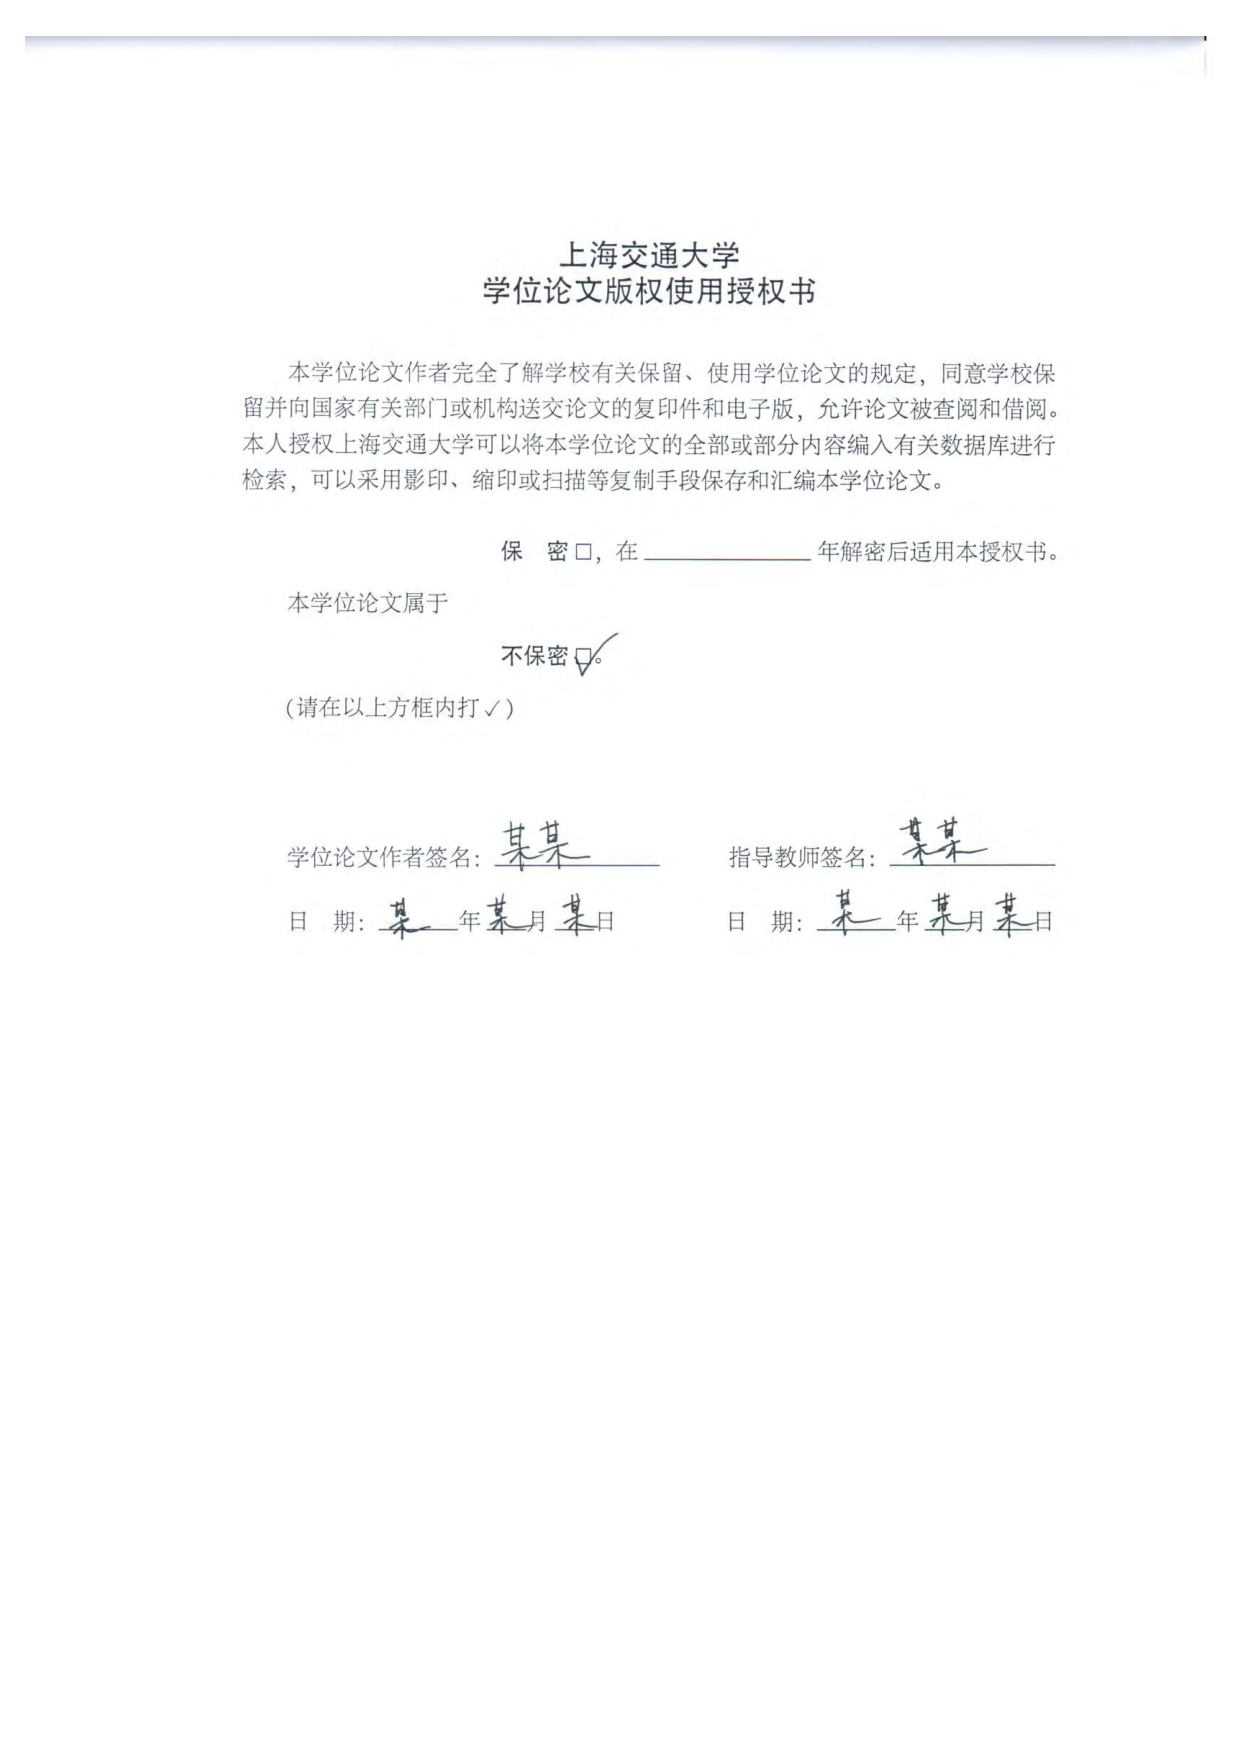
\includepdf{pdf/authorization.pdf}
	\cleardoublepage
\else
\ifsjtu@review\relax
% exclude the original claim and authorization
\else
	\makeDeclareOriginal
	\makeDeclareAuthorization
\fi
\fi
\makeatother


\frontmatter 	% 使用罗马数字对前言编号

%% 摘要
\pagestyle{main}
%# -*- coding: utf-8-unix -*-
% !TEX program = xelatex
% !TEX root = ../thesis.tex

\begin{abstract}

    编程教育吸引了全社会的关注,包括从小学生到计算机专业大学生的各个群体,也包括从商业公司的产品到国家层面的政策指导。
    在线评测系统的诞生给学生们带来了主动练习编程的独特机会。
    只需轻点鼠标,学生们就能方便地访问到在线评测系统上提供的成千上万道题目。
    利用在线评测系统,学生们在自主尝试解决课外的习题时,
    无须付出任何诸如聘请家庭教师之类的人力成本,就能瞬间得到对题目解法的高质量的反馈。
    然而,学生们如果缺乏有经验的老师中指导,常常会不知道应该去尝试在线评测系统上面的哪些题目。
    而有老师自身也是凭借经验挑选题目,缺乏统计数据的支撑。

    近些年的研究表明机器教学方法同样适用于人类学生。
    我们提出一个基于机器教学的智能在线评测系统,借此为学生们定制属于他们自己的训练题库,因材施教。
    我们使用增强学习算法来为学生们设计题库。
    为了解决增强学习算法的训练过程需要大量交互数据的问题,
    我们首先使用真实的在线评测系统的提交记录训练一个用户模型,对学生的水平进行建模,然后让增强学习算法与这个用户模型进行交互。
    实验数据表明,使用我们的用户模型提供的评测指标,我们的推荐算法表现优于基准算法以及人类教师。

\keywords{\large 编程教育 \quad 在线评测系统 \quad 增强学习 \quad 机器教学 \quad 机器学习 \quad 推荐系统}
\end{abstract}

\begin{englishabstract}

    Programming education has attract attention of the whole society,
    from primary school students to computer science majors,
    from products of commercial companies to nation-level policy guidance.
    The invention of online judges brought students a unique opportunity of practice programming proactively.
    Thousands of problems are easily accessible to students on online judges within a single click,
    where they can have consistent feedback instantly without any cost of manpower like private tutors
    whenever they attempt to solve an extracurricular problem.

    However, students without advice of experienced teachers often do not know which problems to do.
    Experienced teachers themselves pick problems in an ad-hoc manner,
    lacking the support of data and statistical analysis.

    Recent researches show that machine teaching techniques can also apply to human students.
    We propose to build an intelligent online judge system with machine teaching techniques
    so that it can help students to find their own optimal problem set.
    We use a reinforcement learning algorithm to design the problem set.
    To tackle with the requirement of the large number of interactive data
    during the training process of the reinforcement learning agent,
    we firstly fit a user model that captures students mindset using submission records from real-world online judges,
    then let the reinforcement learning agent interact with the user model.
    Experiment data shows that our algorithm outperforms baseline methods and human teachers,
    based on metrics of our user model.

\englishkeywords{\large Programming Education, Online Judge, Reinforcement Learning, Machine Teaching, Machine Learning, Recommendation System}
\end{englishabstract}



%% 目录、插图目录、表格目录
\tableofcontents
\listoffigures
\addcontentsline{toc}{chapter}{\listfigurename} %将插图目录加入全文目录
\listoftables
\addcontentsline{toc}{chapter}{\listtablename}  %将表格目录加入全文目录
\listofalgorithms
\addcontentsline{toc}{chapter}{\listalgorithmname} %将算法目录加入全文目录

% %# -*- coding: utf-8-unix -*-
\begin{nomenclaturename}
\label{chap:symb}

\begin{longtable}{rl}
$\epsilon$     & 介电常数 \\
 $\mu$ 		& 磁导率 \\
 $\epsilon$     & 介电常数 \\
 $\mu$ 		& 磁导率 \\
 $\epsilon$     & 介电常数 \\
 $\mu$ 		& 磁导率 \\
 $\epsilon$ 	& 介电常数 \\
 $\mu$ 		& 磁导率 \\
 $\epsilon$     & 介电常数 \\
 $\mu$ 		& 磁导率 \\
 $\epsilon$     & 介电常数 \\
 $\mu$ 		& 磁导率 \\
 $\epsilon$     & 介电常数 \\
 $\mu$ 		& 磁导率 \\
 $\epsilon$ 	& 介电常数 \\
 $\mu$ 		& 磁导率 \\
 $\epsilon$     & 介电常数 \\
 $\mu$ 		& 磁导率 \\
 $\epsilon$     & 介电常数 \\
 $\mu$ 		& 磁导率 \\
 $\epsilon$     & 介电常数 \\
 $\mu$ 		& 磁导率 \\
 $\epsilon$ 	& 介电常数 \\
 $\mu$ 		& 磁导率 \\
 $\epsilon$     & 介电常数 \\
 $\mu$ 		& 磁导率 \\
 $\epsilon$     & 介电常数 \\
 $\mu$ 		& 磁导率 \\
 $\epsilon$     & 介电常数 \\
 $\mu$ 		& 磁导率 \\
 $\epsilon$ 	& 介电常数 \\
 $\mu$ 		& 磁导率 \\
 $\epsilon$     & 介电常数 \\
 $\mu$ 		& 磁导率 \\
 $\epsilon$     & 介电常数 \\
 $\mu$ 		& 磁导率 \\
 $\epsilon$     & 介电常数 \\
 $\mu$ 		& 磁导率 \\
 $\epsilon$ 	& 介电常数 \\
 $\mu$ 		& 磁导率 \\
 $\epsilon$     & 介电常数 \\
 $\mu$ 		& 磁导率 \\
 $\epsilon$     & 介电常数 \\
 $\mu$ 		& 磁导率 \\
 $\epsilon$     & 介电常数 \\
 $\mu$ 		& 磁导率 \\
 $\epsilon$ 	& 介电常数 \\
 $\mu$ 		& 磁导率 \\
 $\epsilon$     & 介电常数 \\
 $\mu$ 		& 磁导率 \\
 $\epsilon$     & 介电常数 \\
 $\mu$ 		& 磁导率 \\
 $\epsilon$     & 介电常数 \\
 $\mu$ 		& 磁导率 \\
\end{longtable}

\end{nomenclaturename}
 % 主要符号、缩略词对照表

\mainmatter	% 使用阿拉伯数字对正文编号

%% 正文内容
\pagestyle{main}
%# -*- coding: utf-8-unix -*-

%\bibliographystyle{sjtu2}%[此处用于每章都生产参考文献]
\chapter{Introduction}
\label{chap:intro}

TODO: introduction


%# -*- coding: utf-8-unix -*-
% !TEX program = xelatex
% !TEX root = ../thesis.tex

\chapter{Background}
\label{chap:background}

\section{Online Judge}
    
    \subsection{Programming Education}

        As we walk into a century surrounded by all kinds of computing devices,
        programming skill gains more and more attention. \todo{cite}
        Universities used to teaching programming to merely computer science majored students,
        but more and more of them are opening the course to all.  \todo{cite}

        One part of programming education is mastering one programming language.
        Mechanisms of modern computers may be too complicated for non computer science majored students to learn,
        but thanks to the abstractions of processors, operating systems, and high-level programming languages,
        it becomes easier and easier to program computers to do what users want.
        The most popular high-level programming languages includes C++, Python, Java, and so on. \todo{cite}
        Instead of dealing with registers and memory addresses using processors' instruction set,
        high-level programming languages bring up concepts like variables, arrays, expressions, loops, functions,
        threads, processes, and other computer science abstractions.

        The other part of programming education is learning programmatic thinking, in other words,
        algorithms and data structures, especially for computer science majored students.
        There may be several solutions to the same problem, but taking different approaches costs differently.
        An $O(n\log n)$ algorithm better scales to a larger input comparing to an $O(n^2)$ algorithm.
        Programming also helps students cultivate thinking skills.
        There are mind sports specially focus on algorithms.
        For instance, ACM International Collegiate Programming Contest (\emph{ACM-ICPC}) is an annual
        competitive programming competition among the universities of world.
        In 2017, 49,935 students from 3,098 universities in 111 countries participated. \todo{cite (wiki)}
        Companies value this kind of thinking skills, as well.
        It is a common practice for companies to ask algorithm puzzles when interviewing candidate programmers.

        Higher level coursers in computer science, like Networking, Machine Learning, and so on,
        need students to be able to express their mind in code.
        Therefore, It is crucial for students to master programming at the very beginning of study,
        which puts challenges to entry-level courses, such as Programming Language, Data Structures, and so on.

        Like any other skills, both mastering one programming language and learning programmatic thinking
        require students to practice repeatedly.
        Important ways of these entry-level courses to help students master programming are assignments and exams.
        Problems in the assignments and exams are likely to be tasks asking students to write code.
        Graphics interfaces, keyboard and mouse inputs, video and audio outputs, networking connections,
        reading from and writing to disks, and so on, are common operations what programs in end-users' computers would have,
        but it would be too much burden for starters.
        Because these problems are for educational purpose only, the tasks are simplified from the real world ones.

        Descriptions of these problems are simple and neat. The tasks are idealized.
        Students do not need to deal with neither incorrect inputs nor malicious data.
        Problems are algorithmic in nature, thus there is no need to consider human-computer interaction.
        Memory is assumed to be large enough for the problems, therefore students can avoid disk operations
        and keep everything in memory.
        In a word, these assignments and exams ask students to write code that focus on the ``computing'' part of programming.

        After students finish the tasks, there need to be some ways to give them feedback, at least,
        tell students whether their solution is correct or not.
        Traditionally, grading programming solutions had no difference from grading calculus homework.
        And the emerge of online judges two decades ago enabled more efficient grading.
        
    \subsection{Manual Grading}

        Before the appearance of online judges, teachers needed to grade programming solutions manually.
        First, students handed in their solutions.
        Then, graders (either the professor himself/herself or the teaching assistants)
        would read the code and give marks based on their professional judgment.
        Manual grading is still a common practice nowadays in other subjects, such as mathematics and physics.
        Though widely used, its effectiveness is still affected by several non-controllable factors
        and has significant drawbacks. \cite{Kurnia2001}

        \subsubsection{Discouragement of Alternative Solutions}

            When the teachers are sketching a problem, they have a standard solution in mind.
            So when graders are grading students' solutions, they expect the code to be similar to
            the standard solution that they were told.
            However, it is likely that there are several alternative solutions to the same problem
            with the same complexity if not better.
            For instance, suppose an assignment can reduce to a minimum spanning tree problem
            and the author expects the Prim algorithm.  \todo{cite Prim}
            A student might turn in a solution with Kruskral algorithm which is also an algorithm that
            solves the minimum spanning tree problem.  \todo{cite Kruskral}
            In this case, if the grader is not aware of Kruskral algorithm, the grader might give a wrong verdict
            because Kruskral algorithm looks completely different from Prim algorithm, i.e. the standard solution.
            Notice that this is not the fault of the grader, because the grader might be a teaching assistant
            who is only expected to be familiar with the standard solution.
            Neither is this the fault of the problem author, because there can be any number of alternative solutions
            and the author cannot enumerate them all.
            Nor should we blame the student.
            In the contrary, students with alternative solutions should be encouraged.

        \subsubsection{Slow Grading}

            Grading a programming solution can takes a long time.
            Unlike a solution to mathematics homework in which students will explain their thinking process
            step by step in natural language,
            a solution to programming problem is code in some programming language which is designed
            for machines to compile, instead of letting humans to read.
            The grader have to read the code carefully in order to understand the solution.
            Then they need to look into details trying to find potential mistakes.
            Consequently, the grading process can be very slow.

        \subsubsection{Inconsistency}

            The same solution might have different scores if it is graded by different graders.
            For example, some graders know more than the standard solutions,
            and thus justify the alternative solutions.

            Even for the same grader to check the same solution at different times might lead to different results.
            For instance, at the beginning of grading, the grader might be very patient
            and carefully reason about each line of code.
            However, after hours of grading, the grader could feel tired and distracted
            and might want to finish grading as soon as possible.
            In this case, the grader might only check if the solution matches some patterns of the standard solution.

            Needless to say, the same solution is likely to have completely different verdicts
            depending on who the grader is and what status he or she is in.

        \subsubsection{Ignorance of Details Mistakes}

            Because of understanding students' solution costs graders lots of energy,
            subtle mistakes hidden in details often escape from being found.
            For example, supposing the standard solution is Floyd algorithm, \todo{cite}
            the grader might expect students' solutions to have two kinds of patterns:
            three nested loops and a dynamic programming equation.
            However, the solution might mixing up the permutation of the three loop variables,
            which makes the algorithm no longer correct.
            The grader might not be able to find such subtle an error.
            \todo{correct and incorrect floyd code}

        \subsubsection{Low Scalability}

            One of the hot topics computer scientists deals with is scalability.
            Ironically, manually grading programming assignments doesn't scale well.
            The increasing in either students or problems significantly add burden to graders.
            Apparently the total number of problems the professor can assign is proportional to
            the number of teaching assistants, and is inversely proportional to the number of students.
            Although the department could employ more teaching assistants to avoid the intolerable grading time,
            the inconsistency caused by different graders would become more and more disturbing.

        \subsubsection{Long Feedback Time}

            Manual grading takes graders a long time to justify the correctness of students' solutions,
            in the mean time, the feedback time of students is even longer.
            Counting the time starting from the moment a student finishes the solution to the moment
            the student knows about the verdict, it usually takes days if not weeks to have the feedback.
            Days after writing the code, the student might need to spend extra time to recover
            the thinking process when he or she was solving the problem.
            Sometimes, students just fail to go back to the mindset then, and thus the lessons learned from
            the assignment mistakes would be discounted.

    \subsection{Automatic Grading}

        The invention of online judges brought the idea of automatic grading, that is,
        letting a computer program to determine the correctness of programming assignments.
        In order to transit from manual grading to automatic grading,
        teachers need to formalize the grading process in a way that a program grader are easy to handle,
        otherwise computer scientists need to build a strong artificial intelligence
        just to grade some homework and exams, which is not yet possible for now and wastes its talent.

        \subsubsection{Grading Process}

            Instead of writing code on pieces of paper, students need to write code on a computer
            and hand in the source code as it is to the online judge.
            In fact, submitting the source code makes more sense than handing in pieces of paper.
            Students can avoid compilation errors by compiling the source code,
            which would be a trivial mistake but often caught in hand-written code.
            Further more, students can convenience themselves the code is correct by running the code
            over several inputs and they can even debug it if they find something not working as expected.

            To simplify programming tasks, avoiding fancy human-computer interaction
            and complicated input/output operations, online judges require the problem author and students
            to behave within some conventions:

            \begin{itemize}
                \item The solution code should compile and run (or can be interpreted for interpreted languages).
                \item The program should read data from the \emph{standard input}
                      and write answers to the \emph{standard output}.
                \item The program should not have any other input/output operations, such as writing a file,
                      connecting to the network, and so on.
                \item The program should terminate within certain \emph{time limit} and \emph{memory limit}.
                \item The program should not have any malicious behaviors.
                \item The problem author should specify the \emph{input format} and the \emph{output format}.
                \item The problem author should specify \emph{the range of input data}.
                \item The problem author should specify the time limit and memory limit.
                \item The problem author should make several \emph{testcases} along with the problem.
                      Each testcase consist of input data and output data.
                      Output data is the answer as if produced by a correct program.
                      The input and output data should be consistent with the input and output format
                      specified in the problem description.
            \end{itemize}

            The problem author can give several sample testcases in the problem description
            to help students understand the problem setting and the input/output format.
            Students can also use it to verify if there is obvious flaw in the solution.
            However, there should be a set of secret testcases that students cannot access.
            Otherwise, the students merely need to write a program that prints the corresponding
            standard answer according to the input.

            Students' solution presumes to be correct if it can pass all testcases.
            If the program passes only part of the testcases, the online judge can also gives partial credits.
            With this convention in mind, the grading process becomes programmatic.

            \begin{enumerate}
                \item Students submit the source code to the online judge.
                \item The online judge compiles the source code (if it is a compiled language).
                \item The online judge runs the program with the input the problem author designed.
                \item The online judge checks if the program terminates within the specified
                      time and memory constraints and does not have any malicious behaviors.
                \item The online judge compares the program output to the corresponding output
                      the problem author designed.
                \item The above three steps repeats until all of the testcases have been examined.
                \item The online judge either claims the solution to be correct if the program
                      has passed all testcases or gives partial credits.
            \end{enumerate}

            A flawed solution might be able to pass one or two testcases, but the chance of
            passing all testcases is low enough if the testcases was carefully designed.

            This kind of automatic grading process can also detect incorrect algorithmic complexity.
            For example, it is easy for an $O(n\log n)$ solution to terminate within one second
            on a $n=10,000$ input, but not likely for an $O(n^3)$ one.
            The same idea applies to space complexity due to the memory limit
            specified in the problem description.

        \subsubsection{Advantages}

            The automatic grading process addresses the flaws in manual grading.

            By definition of correctness, any solution that solves a problem correctly
            is able to pass all the testcases.

            Automatic grading is at least dozens of times faster than manual grading.
            Assuming the time limit for each testcase is one second and there are ten testcases in total,
            the maximum run time for a student's solution would be ten seconds.
            There are some extra times costs by the automatic grader, including
            compiling the student's solution, comparing the program output to the standard answer,
            and some other necessary operations of the automatic grader.
            Therefore, in the worst case,
            the grading process can be done in a little bit more than ten seconds in total.
            Typically, the whole process should finish in seconds,
            since a correct solution is expected to run significantly faster than the time limit.

            With such fast grading speed, students can get the feedback almost instantly.
            Hence, they are quite clear about the code they wrote just now, and thus easier to 
            reason about the mistakes if the online judge did not give them full credits.

            Notice that the automatic grading process does not require
            the teacher or any teaching assistants presenting
            once the problem author has published the problem.
            The interaction only happens between students and the online judge.
            Without human being involving in the grading process,
            lots of uncertainties are eliminated,
            because the execution of the grading program is determined.
            As long as the machine running the automatic grader has sufficient computing power,
            the running result will be the same.
            The maintainer of the online judge simply need to
            make sure the computer is dedicated for automatic grading.
            The automatic grading program would not have any `mood', nor does it feel tired.
            Consequently, it will produce consistent verdicts.

            Clearly, the increase in the number of students and problems does not add burdens to the online judge.
            It just reduces the idle time of the automatic grader.
            At the worst case, new submissions start to accumulate and waits in queue.
            In this case, simply buying more machines and running more automatic graders
            suffice to keep a short enough waiting time.
            The costs of new computers is cheaper than paying stipend to teaching assistants,
            not to mention that lots of departments have spare servers to use.

    \subsection{Online Judges}

        Due to its overwhelming superiority,
        universities widely integrate online judges with programming-related courses \cite{Li2005}.
        There are dozens of popular online judges.
        Some of them are famous world-wide, such as CodeForces, TopCoder, SPOJ, uVA, and so on. \todo{cite}
        Online judges can roughly divide into three categories.

        One is maintained by universities, such as POJ, HDU, and so on. \todo{cite}
        The university's ACM-ICPC participants actively train on these online judges.
        In addition, these online judges also serve programming courses.
        Teaching assistants hand out homework assignments and organize exams on online judges.

        Another is maintained by high schools
        or retired Olympiad in Informatics (\emph{OI}) participants,
        such as LibreOJ, and so on. \todo{cite}
        Because most high schools do not teach programming systematically,
        the only purpose of these kind of online judges is their internal OI training.

        The last category is operated by commercial companies. \todo{cite; TODO: marong's OJ}
        LeetCode, for example, focus on the interview problems ask by big companies.
        Users need to pay for the full problem set and solutions with high quality explanations.
        In China, the market of private tutoring on competitive programming competitions is getting larger.
        Some commercial companies build online judges, compose series of problems, organize contests,
        and teach lessons for their paid customers.

        Interestingly, almost all online judges share the same convention mentioned in previous subsection.
        Different online judges have their own characteristics as well.

        \subsubsection{Design of Online Judges}

            Online judges usually have a web interface.
            The advantage of using a web interface over native graphics interface is that
            it can easily support different platform.
            Unlike traditional applications, each operating system has a large share of users of online judges.
            This might be because Windows, Linux, and macOS are all very popular among programmers.
            In addition, some of competitive programming competitions encourages the usage of Linux,
            such as Chinese National Olympiad in Informatics (\emph{NOI}).  % site: NOI Linux article
            Since all operating systems have web browsers,
            users do not need to install extra software to use the online judge.
            Some active participants of ACM-ICPC or OI even use mobile web browsers on their smart phones
            to read problems on online judges and think about them in their spare time.

            Users need to register an account on the online judge before they can submit their solution to it.
            Since each solution is tied to an account, online judges can easily show statistics,
            like which problems the user have solved, which problems the user has tried but not ye solved.
            Users can design their own training schedule according to these statistics.
            It also enables computer scientists to create models for users and
            then uses artificial intelligence to design the training schedule for users.

            Once users submit a solution through the web interface,
            the online judge keeps the submission in the database,
            and assign an automatic grader to grade the solution.
            The result of an submission usually can be the following ones:

            \begin{description}
                \item[Accepted] The submitted code has passed all the testcases.
                \item[Partial Credit] The submitted code has passed part of the testcases.
                \item[Compilation Error] The submitted code has failed to compile.
                \item[Wrong Answer] The submitted code has produced incorrect answer on some testcases.
                \item[Runtime Error] The submitted code has exited with non-zero exitcode unexpectedly
                                     when running some testcases.
                \item[Time Limit Exceeded] The submitted code has not terminated within the specified time limit
                                           when running some testcases.
                \item[Memory Limit Exceeded] The submitted code has tried to allocate more memory than the
                                             specified memory limit when running some testcases.
            \end{description}

            In addition to the result, online judges also display two important factors:
            the total running time and the maximum memory usage,
            which indicates the performance of a solution.

            Online judges can run multiple automatic graders on several machines or
            on a machine with multiple processor cores.
            Previous subsection has described how a automatic grader works.

        \subsubsection{Security Concerns}
            \todo{cite security papers}

            The code automatic graders compile and run is submitted by users from the Internet
            which is untrusted and can even be malicious.
            Therefore, the design of online judges must include serious security concerns.

            The very basic protection over the file system would be running the submitted code
            with a non-privileged user in a \texttt{chroot}ed environment
            along with appropriate Linux file system permission,
            preventing malicious source code from reading sensitive configuration file of the online judge
            or tampering with system files.
            Since the submitted code are asked to communicate only through standard input/output,
            any attempts to open a file would be suspicious.
            Linux API \texttt{setrlimit} can set resource limits for the submitted code,
            including CPU time, memory size, the number of opened files, the number of threads, and so on.

            Some automatic graders uses \emph{ptrace} series of Linux APIs to intercept system calls to
            achieve more accurate control over the execution of the submitted code.
            If students' program tries to invoke a forbidden system call or with undesired arguments,
            the automatic grader will immediately kill the process and give ``Runtime Error'' verdict.

            Another technology online judges use to further improve security is \emph{AppArmor}
            which is a Linux kernel enhancement to confine programs to a limited set of resources.
            It can mediate file access, library loading, execution of applications, coarse-grained network,
            capabilities, \texttt{ptrace}, and so on.
            \todo{cite https://wiki.ubuntu.com/Security/Features}

            Although these constraints help improve security,
            it can sometimes block the execution of a benign program,
            especially if the online judge supports variety of programming languages.
            For instance, the interpretation of a Java source code requires the permission to read
            Java library files and the ability to spawn threads for the just-in-time (\emph{JIT}) compiler to run.
            Therefore, the system administrator of a online judge need to carefully tune the security policy configuration.
            Too much constraint will forbid a benign program.
            Too loose policy might expose the risk of security breach.
            It requires the system administrator to be familiar with the compiler and the execution runtime
            of each programming language to write a appropriate security policy,
            which is not feasible for most online judge organizers.
            \todo{snapshot of programming languages on codeforces}

            Recently, \texttt{cgroups} and Linux namespaces features enables operating system level virtualization.
            Container technologies like \emph{LXC} and \emph{Docker} make limiting resources easier.
            Instead of writing detailed security policy,
            the system administrator of a online judge simply need to specify the coarse resource limits.
            The execution of malicious code is tolerable inside the container,
            because the malicious code can at best corrupt the operating system inside the container
            which is isolate from other containers and the host operating system.
            Containers are lightweight as the spawn time is milliseconds and
            there is no overhead of real hardware virtualization.

            Keep in mind that containers are merely isolation provided by Linux kernel.
            Containers and the host share the same kernel.
            Exploiting kernel vulnerabilities might result in the malicious program escaping from the container.
            For an extra level of security,
            system administrators might run the automatic grader container inside some virtual machine hypervisor.
            \todo{diagram of different layers of isolation}

        \subsubsection{Contests}

            Contest is an important feature of online judges.
            Some online judges, like CodeForces, regularly organize contests,
            attracting thousands of participants of competitive programming competitions.

            A contest consists of a set of problems
            which are usually kept secret before the contest starts.
            A typical contest lasts a few hours.
            Participants can solve the problem set on their own in arbitrary order.
            There is a scoreboard displaying real-time score of all participants.
            The scoring rule varies.
            Most of scoring rules sort the scoreboard by the number of accepted solution.
            In order to rank among participants who has solved the same number of problems,
            some rules take the sum of submission time into account, as the second sort key.
            The ACM-ICPC rule also add extra time penalty to each failure submission.
            The OI rule values partial credits.
            The total score is the sum of credits of all problems, ignoring submission time.

            Ranking system is a great stimulation for participants.
            Online judges with ranking systems update each participants ranking score
            after the contest has finished.
            The ranking systems are usually variants of the Elo rating system. \todo{cite elo, tc, cf}
            It takes two factors into account:
            the participant's current ranking, and the ranking of other participants.
            It roughly reflects a participant's level.
            \todo{snapshot of cf ranking}

            The contest feature can also serve as other purpose.
            For example, teachers can hold a exam on the online judge
            and ask students to take the exam on a computer room in a planned time.
            Another useful variant of the contest feature is homework.
            Teaching assistants can hand out the problem set on the online judge,
            set the start and end date (which usually spans days or a few weeks).
            The scoreboard precisely shows whether a student has finished all the assignments.

        \subsubsection{Virtual Judge} \todo{cite; TODO: diagram of the delegation process}

            High quality problems span different online judges.
            Sometimes, students might need to register a new account on a newly visited online judge
            just in order to solve a few assignments.
            Sometimes, tutors of competitive programming competitions might want to organize an exam
            of which problems are from different online judges,
            some of which does not even have a contest feature.
            To deal with these issues, the virtual judge creates a problem-centric platform,
            breaking the boundary of different online judges.

            The ``virtual'' judge is not a ``real'' judge in the sense that it does not own any problems,
            nor does it run any automatic graders.
            It acts like a proxy between students and different online judges.
            The virtual judge has a web crawler that retrieves problem descriptions from different online judges.
            Students can then read all problems across different online judges within the same website.

            Students only need to register one account on the virtual judge.
            The virtual judge has several proxy accounts on each online judge.
            When students submit the code at the virtual judge with their own account,
            the virtual judge automatically submit the code to the corresponding online judge
            with the proxy accounts.
            Then, the web crawler keeps watching the status pages of these delegated submission
            until the result is determined.
            Finally, the virtual judge store the result fetched by the web crawler to its own database
            and show the result to students.

            The virtual judge also provides a contest feature.
            It does not require the upstream online judge to have a contest feature.
            The virtual judge submit a source code in a contest to the upstream online judge
            as if it is a normal submission.
            The service logic of contest, like submission time period and time penalty, is handled
            by the virtual judge itself.

        \subsubsection{Encouragement in Students' Proactive Participation}

            Once a problem is published on a online judge,
            it is likely that it will always be there in the future,
            because it does not make much sense to take down a problem.
            Therefore, students can see thousands of problems on the online judge.
            If they are willing to try to solve them,
            there is nothing to stop them from doing it.
            They can submit their solutions,
            and the online judge will tell whether it is correct or not.
            It will not require any extra manpower to grade the solution.
            In fact, active participants of competitive programming competitions usually proactively
            train themselves on online judges.
            They even take part in regular contests which online judges organizes.

            With thousands of problems available online, comes another issue:
            students submerged by an overwhelming number of problems usually feel lost
            if they does not have an experienced teacher to tell them which problems to solve.

            Some online judges try to address this issue by creating lists of problems
            categorized by the knowledge components that problems need.
            These lists are usually created by teachers,
            who themselves create the list in a ad-hoc manner
            according to their years of teaching experience.

            Although teachers' experience are precious,
            we must notice that each student is unique.
            They have different mindsets, different ways to understand knowledge,
            and different levels of knowing each knowledge components.
            We expect with the development of artificial intelligence
            and exploitation of millions of submissions data,
            online judges can design unique training problem set for each student.


\section{Machine Teaching}

    Machine learning and deep learning have showed their great accuracy and generalization capability
    in many areas including computer visions, natural language processing, speech recognition, and so on.
    However, to train a machine learning model requires experts in machine learning.
    The demand of machine learning model exceeds the supply of ``teachers'' that are able to teach machines.
    In contrast to the machine learning field which focuses on performances like accuracy,
    the machine teaching field pays attention to the efficacy of the teachers given the learners,
    enabling more people like data scientists and domain experts to teach machine learning algorithms,
    the number of which can be hundreds of times more than the number of machine learning experts \cite{Simard2017}.

    A ``teacher'' in machine teaching field aim to design the optimal training set $D$
    to teach a given ``learner'' $A$ a specific model $\theta^*$.
    The definition of ``optimal'' varies.
    For instance, it can be the size of the training set.

    \cite{Zhu2018} views machine teaching as an inverse problem to machine learning.
    Given $D \in \mathbb{D}$ and $A \in \mathbb{A}$, machine learning results in a model $A(D) \in \Theta$.
    Given $\theta^* \in \Theta$ and $A \in \mathbb{A}$,
    there is a subspace $A^{-1}(\theta^*) \subseteq \mathbb{D}$ of training set space. 
    Training $A$ with training set inside $A^{-1}(\theta^*)$ results in the target model $\theta^*$.
    \todo{graph}

    Although a ``teacher'' knows $\theta^*$,
    it is likely that the ``teacher'' cannot directly ``hard wire''the ``learner''
    because they are usually not the same type of entities.

    Machine teaching applications can look quite different depending who teaches whom.

    \subsection{Human teacher teaches machine learner}

        Machine learning experts who have deep understanding of the learner algorithm
        and human experts in the learner's domain can design the optimal training set
        boosting the training efficiency of the learner.

        Consider a one-dimension threshold classifier.
        The input distribution is uniform over the interval $[0,1]$.
        Denote the true threshold as $\theta^*$.
        The label is binary and noiseless: $y := \bm{1}_{x \geq \theta^*}$.

        Passive learning receives $n$ training items
        $x_1, x_2, \cdots, x_n \sim U[0,1]$ with $y_i = \bm{1}_{x \geq \theta^*}$.
        It can be shown that with large probability a consistent learner (one that makes zero training error)
        incurs a generalization error $\left|\hat{\theta} - \theta^*\right| = O(n^{-1})$ \cite{Zhu2018}.
        The uncertainty of the decision boundary is defined by the innermost pair of negative and positive samples.
        Equivalently, archiving $\epsilon$ error requires $n \geq O(\epsilon^{-1})$ training data.

        A human teacher knows $\theta^*$ can construct a training set containing only two items
        that are $\epsilon$ apart with $\theta^8$ in the middle.
        Training on this two-item training set results in $\epsilon$ generalization error for any $\epsilon$.

        Study shows that in the case that human teacher is not able to give the optimal training set,
        machine teaching allows the machine student to ``teach the human how to teach'' \cite{Suh2016}.

    \subsection{Machine teacher teaches machine learner}

        An adaptive spam filter $A(D)$ are constantly re-train over time on training set $D$ to accommodate
        the changing legitimate content and the variants of spams.
        The machine learner can be a malicious program that sends specially designed emails
        to the spam filter to manipulate the threshold from $\hat{\theta}$ to some nefarious $\theta^*$ instead,
        such that certain spam emails can get pass the filter \cite{Alfeld2016}.
        The machine learner changes the training set of the spam filter subtly by $\delta$ to avoid detection \cite{Mei2015}.
        The attacking problem can be formalized as:

        \begin{equation*}
        \begin{aligned}
            \min_{\delta, \hat{\theta}} \quad &
            \left\lVert\hat{\theta} - \theta^*\right\rVert + \eta \left\lVert\delta\right\rVert \\
            \textrm{s.t.} \quad & \hat{\theta} = A(D+\delta)
        \end{aligned}
        \end{equation*}

    \subsection{Machine teacher teaches human learner: Education}

        Every human student is unique.
        They have different mindsets, different skill sets, and different mastery over knowledge components.
        Machine teaching provides a unique approach to design the optimal lessons for individual students.

        Machine teaching explicitly assumes a cognitive model $A$ of students.
        Given lessons $D$, we can compute the resulting cognitive state $A(D)$,
        and then evaluate the test score via an appropriate teaching risk function $\rho(A(D), \theta^*)$
        whose minimum is at $\theta^*$.
        In other words, machine teaching treats the human learner as a ``transparent box.''

        Although having a correct cognitive model is a strong assumption,
        machine teaching with inaccurate cognitive model still works on humans \cite{Whitehill2017}.
        In the work of \cite{Patil2014},
        researchers assumes a limited capacity retrieval cognitive model of human learners
        in a one-dimension classification task.
        Human testers trained on the training set the machine teaching method designed
        has statistically significantly better test accuracy than who trained on a random training set.


\section{Logistic Regression}

    Tom Mitchell gives a formal definition of machine learning:
    ``A computer program is said to learn from experience $E$ with respect to some class of tasks $T$
    and performance measure $P$ if its performance at tasks in $T$, as measured by $P$, improves with experience $E$.''
    \cite{Mitchell1997}
    Machine learning relies on experience.
    Depending on what experience is like, machine learning tasks can be broadly classified into two types:
    supervised learning and unsupervised learning.

    A supervised learning task learns a function based on example training data.
    In supervised learning, each piece of training data consist of a pair of input vector
    and the desired output, called \emph{label}.
    A supervised learning algorithm goes through the training data and infers the function
    which can be used to predict new examples.
    In contrast to the performance on the training data,
    researchers pay more attention to the ability of the model to correctly predict unseen data,
    i.e. the capability of generalization.
    Sometimes, predictions on the input training data can greatly outperform that on unseen data.
    In this case, the model is overfitted, meaning that the model has ``memorized'' the training data
    but did not ``learn''.

    Logistic regression is a widely used supervised learning model.
    The output of logistic regression is a probability for a label to belong to a given data.
    The label is binary discrete.
    In other words, a data point can only be either a positive sample or a negative sample.
    Given input vector $x$ and some coefficients $w$,
    logistic regression learns a function of the following form:

    \begin{align*}
        P(y=1 | x;w) &= \frac{1}{1+\exp(-w^Tx)} = \sigma(w^Tx)\\
        P(y=0 | x;w) &= 1-P(y=1 | x) = 1-\sigma(w^Tx)
    \end{align*}

    where

    \[
    \sigma(x) = \frac{1}{1+\exp(-z)}
    \]

    is the logistic function (or the \emph{sigmoid} function).
    It is an ``S''-shaped function, mapping $w^Tx$ to $[0,1]$
    so that we can interpret $\sigma(w^Tx)$ as a probability.
    Training a logistic regression model is a process that tries to find $w$ so that
    $P(y=1 | x)$ is large for the input vector $x$ that belongs to the positive class,
    and symmetrically, $P(y=0 | x)$ is large for the input vector $x$ that belongs to the negative class.

    For a set of training examples with binary labels $\left\{ (x^{(i)}, y^{(i)} | i = 1, 2, \cdots, m) \right\}$,
    the loss function, i.e. the log likelihood, is

    \[
    l(w) = -\sum_{i=1}^m \left( y^{(i)}\log\left(\sigma(w^Tx^{(i)})\right) + (1-y^{(i)})\log\left(1-\sigma(w^Tx^{(i)})\right) \right)
    \]

    It can be prove \cite{Ng2000} that the gradient of the loss function is

    \[
    \nabla_w l(w) = \sum_{i=1}^m x^{(i)}\left(\sigma(w^Tx^{(i)}) - y^{(i)}\right)
    \]

    We can derive the update rule of the stochastic gradient ascent from this:

    \[
    w_j := w_j + \eta \left( y^{(i)} - \sigma(w^Tx^{(i)}) \right) x_j^{(i)}
    \]

    where $\eta$ is the learning rate.

    In other words, the computation of both the logistic regression model and its gradient is fast.
    Consequently, logistic regression model is widely adopted in the industry,
    especially where computation time is limited, such as click-through-rate estimation and recommendation systems.
    \todo{cite}

    \subsection{Kernel Tricks}

        The definition of logistic regression shows that it's a linear model
        because the relation of the input vector $x$ and the coefficients $w$ is a linear combination.
        However, the capability of a linear model is limited.
        It cannot discover the relationship between different input features,
        i.e., different dimensions of the input vector.

        For instance, in a recommendation system, there is usually three types of features: \cite{Ricci2011}

        \begin{description}
            \item[User Features] Each user may have a set of attributes.
                For example, user demographic includes users' age, gender, and so on.
                Some of these features may be filled by the user, like education level.
                And others can be inferred by their behavior, such as their interested music genres.
            \item[Item Features] Items are products which the recommendation system would like to recommend to users,
                such as books on an online shop.
                Items also have a set of characteristics.
                For example, the author of a book.
            \item[Context Features] These features reflects interactions between users and items.
                Some features provide additional information,
                for example, it can be it can be a user's rate on a specific book.
                Others can be derived from user features and item features.
        \end{description}

        To enable a linear model to capture the relations between user features and item features,
        it requires domain experts manually calculating context features.

        Mathematically, the data points are not always linearly separable.
        Kernel tricks enables linear models like logistic regression to capture non-linear regression.

        For all $x$ and $x'$ in the input space $\mathcal{X}$,
        certain functions $k(x, x')$ can be expressed as an inner product $\langle\cdot,\cdot\rangle_{\mathcal{V}}$
        in another space $\mathcal{V}$:

        \[
        k(x, x') = \langle \varphi(x), \varphi(x') \rangle_{\mathcal{V}}
        \]

        where $\varphi: \mathcal{X} \rightarrow \mathcal{V}$ is the feature map.
        The function $k: \mathcal{X} \times \mathcal{X} \rightarrow \mathbb{R}$ is called a \emph{kernel} function.

        For example, consider a two dimension space.
        Data points $(x_1, x_2)$ within a oval are positive samples and others are negative samples.
        In this case, it is not linear separable.
        Consider the feature map $\varphi((x_1, x_2)) = (x_1^2, \sqrt{2}x_1x_2, x_2^2)$.
        Now data becomes linearly separable. \cite{Rai2011}
        \todo{figure}

        The more general kernel is quadratic kernels.
        Consider data point $x = (x_1, x_2, \cdots, x_n)$.
        A quadratic kernel maps $x$ to 

        \[
        \varphi(x) := (1, \sqrt{2}x_1, \cdots, \sqrt{2}x_n, x_1^2, \cdots, x_n^2,
          \sqrt{2}x_1x_2, \cdots, \sqrt{2}x_1x_n, \cdots, \sqrt{2}x_{n-1}x_n)
        \]

        Each new feature uses a pair of the original features,
        therefore, it can capture the interaction between each pair of features.

\section{Factorization Machine}

    \subsection{Limitation of Kernel Tricks}

        Notice that, the linear combination of the transformed feature vector and the coefficients is

        \[
        w^T\varphi(x) = w_0 + \sqrt{2}\sum_{i=1}^n w_ix_i
        + \sum_{i=1}^n w_{ii}x_i^2 + \sqrt{2}\sum_{i=1}^n\sum_{j=i+1}^n w_{ij}x_ix_j
        \]

        In other words, the number of parameters of a $n$-dimension input has $O(n^2)$ dimensions.
        However, it may not work well with recommendation systems.

        The input vector of recommendation systems are usually sparse.
        For example, there can be some one-hot features.
        A one-hot feature may span thousands of dimension.
        There is only one dimension has non-zero value and the others are all zeros.

        The blast of the number of parameters makes the training process inefficient.
        What's worse, in order to learn $w_{ij}$,
        there need to be enough input vectors that satisfy $x_i \neq 0$ and $x_j \neq 0$,
        which usually is not true for all pairs of $i$ and $j$.
        Consequently, the inefficient learning process might eventually result in a ineffective model
        because $w_{ij}$ is noisy.
        It is obvious that this issue will become worse if we want to capture relations of three or more features.

    \subsection{Factorization Machine}

        Factorization machine allows parameter estimation under very sparse data
        where linear regressions with kernel tricks fail. \cite{Rendle2010}

        The model equation for a factorization machine of degree $d=2$ is defines as:

        \begin{equation}
        y(x) := w_0 + \sum_{i=1}^n w_i x_i + \sum_{i=1}^n\sum_{j=i+1}^n \langle \bm{v}_i, \bm{v}_j \rangle x_ix_j
        \label{eq:fm}
        \end{equation}

        where the the model parameters that have to be estimated are:

        \[
        w_0 \in \mathbb{R}, \quad w \in \mathbb{R}^n, \quad \bm{V} \in \mathbb{R}^{n \times k}
        \]

        And $\langle \cdot, \cdot \rangle$ is the dot product of two vectors of size $k$:

        \[
        \langle \bm{v}_i, \bm{v}_j \rangle := \sum_{f=1}^k v_{if}v_{jf}
        \]

        A row $\bm{v}_i$ within $\bm{V}$ describes the $i$-th variable with $k$ factors.
        $k \in \mathbb{N}_0^+$ is a hyperparameter that defines the dimensionality of the factorization.

        The two-degree factorization machine captures all single and pairwise interactions between variables:

        \begin{itemize}
            \item $w_0$ is the global bias.
            \item $w_i$ models the importance of $i$-th variable.
            \item $\langle \bm{v}_i, \bm{v}_j \rangle$ reflects the interaction
                between the $i$-th variable and the $j$-th variable.
        \end{itemize}

        The difference between the factorization machine and kernel tricks is that
        kernel tricks use a independent parameter for each pair of interaction, resulting in $O(n^2)$ parameters,
        but the factorization machine models the interaction by factorizing it, resulting in $O(nk)$ parameters.
        For large enough $k$, the factorization machine is able to express any interaction matrix $\bm{W}$ \cite{Rendle2010},
        therefore, the factorization machine is as expressive as kernel tricks.
        On the other hand, choosing small $k$ restricts the capability of the factorization machine,
        which in turn can reduce the noisy and leads to better generalization under sparsity,
        because there is not enough data to disclose the complicated pairwise interaction.
        \todo{figure like https://www.zhihu.com/question/27043630}

        Although the complexity of calculating the score function of the factorization machine \ref{eq:fm}
        might seem to be $O(kn^2)$ if taking a naive approach,
        transforming the formula in the following manner shows that it can be done in linear time $O(kn)$:

        \begin{align*}
        & \sum_{i=1}^n\sum_{j=i+1}^n \langle \bm{v}_i, \bm{v}_j \rangle x_ix_j \\
        =& \frac { 1} { 2} \sum _ { i = 1} ^ { n } \sum _ { j = 1} ^ { n } \left\langle \bm { v } _ { i } ,\bm { v } _ { j } \right\rangle x _ { i } x _ { j } - \frac { 1} { 2} \sum _ { i = 1} ^ { n } \left\langle \bm { v } _ { i } ,\bm { v } _ { i } \right\rangle x _ { i } x _ { i } \\
        =& \frac { 1} { 2} \left( \sum _ { i = 1} ^ { n } \sum _ { j = 1} ^ { n } \sum _ { f = 1} ^ { k } v _ { if } v _ { jf} x _ { i } x _ { j } - \sum _ { i = 1} ^ { n } \sum _ { f = 1} ^ { k } v _ { if } v _ { if } x _ { i } x _ { i } \right) \\
        =& \frac { 1} { 2} \sum _ { f = 1} ^ { k } \left( \left( \sum _ { i = 1} ^ { n } v _ { if } x _ { i } \right) \left( \sum _ { j = 1} ^ { n } v _ { jf } x _ { j } \right) - \sum _ { i = 1} ^ { n } v _ { if } ^ { 2} x _ { i } ^ { 2} \right) \\
        =& \frac { 1} { 2} \sum _ { f = 1} ^ { k } \left( \left( \sum _ { i = 1} ^ { n } v _ { if } x _ { i } \right) ^ { 2} - \sum _ { i = 1} ^ { n } v _ { if } ^ { 2} x _ { i } ^ { 2} \right)
        \end{align*}

        The two-degree factorization machine can be generalized to a $d$-degree factorization machine:

        \[
        y(x) = w_0 + \sum_{i=1}^n w_ix_i +
        \sum_{l=2}^d\sum_{i_1=1}^n\cdots\sum_{i_{l-1}+1}^n \left( \prod_{j=1}^l x_{i_j} \right)
        \left( \sum_{f=1}^{k_l}\prod_{j=1}^l v_{i_j,f}^{(l)} \right)
        \]

        where the interaction parameters for the $l$-th interaction is

        \[
        \bm{V}^{(l)} \in \mathbb{R}^{n \times k_l}, \quad k_l \in \mathbb{N}_0^+
        \]

        It can be proved that by similar transformation, the computation is still linear. \cite{Rendle2010}

        To sum up, the factorization machine is an efficient algorithm
        that can capture interactions of two or more variables
        and has better generalization under sparsity compared to kernel tricks.
        
\section{Boosted Trees}

        Decision tree is another widely used model for data analysis.

        A decision tree is a binary tree.
        Each node has exactly one parent (except for the only root node) and two children.
        Each internal node split the input subspace into two halves by a certain criteria.
        The leaves represents a category.

        Given a decision tree, the evaluation of a input is quite straight forward.
        At each internal node, decide which children to go by check the criteria.
        Repeat the procedure above recursively until reaching a leaf node.

        Similarly, the interpretation of a decision tree is also straight forward,
        which is its unique advantage over other machine learning algorithms.
        Because each node has a certain criteria,
        drawing the binary tree along with those criteria would give a clear explanation.
        A data analysis service provider can explain the model to the buyer by visualizing
        the decision tree without the need for the buyer to know statistic or machine learning knowledge.
        \todo{example figure}

    \subsection{XGBoost}

        Gradient boosting is a machine learning technique,
        which produces a prediction model in the form of an ensemble of weak prediction models.
        Gradient boosting is typically used with decision trees of a fixed size as base learners.
        For this special case, \cite{Friedman2001} proposes a modification to gradient boosting method
        which improves the quality of fit of each base learner.

        XGBoost is a scalable machine learning system for tree boosting. \cite{Chen2016}

        \todo{make this section look better}

\section{Recurrent Neural Networks}

    Recurrent neural networks are a family of neural networks for processing sequential data.
    Traditional neural networks assumes the inputs are independent of each other,
    thus they cannot find connections inside the input of sequential data.
    In order to process sequential data, the model need to know context information.
    For example, predicting the next character in a sentence would heavily depend on
    characters came before it.

    Recurrent neural networks ``recurrently'' compute the output of current step
    depending on the calculation of the previous step.
    In other words, recurrent neural networks have internal states
    that memorize the context information between steps.

    \subsection{Vanilla Recurrent Neural Networks}

        \todo{RNN diagram (ref:http://www.wildml.com/2015/09/recurrent-neural-networks-tutorial-part-1-introduction-to-rnns/)}

        The diagram shows the unfold of the vanilla recurrent neural network.

        \begin{itemize}
            \item $x_t$ is the input at time step $t$.
                Interestingly, inputs may not be needed for each time step.
                For instance, in the image captioning task,
                the input presents only at the first time step which is the input image.
                The recurrent neural network then produce the sentence step by step and character by character.
            \item $h_t$ is the hidden state at time step $t$.
                Its computation depends on the previous hidden state and input of the current time step:
                $h_t = f(Ux_t + Wh_{t-1})$.
                Thus, it memorizes the context until so far.
                The activation function $f$ is usually a nonlinear function like $\tanh$ or $\mathrm{ReLU}$,
                which gives the recurrent neural network the capability of fitting a nonlinear function.
                The initial state $h_0$ is usually initialized to all zeros.
            \item $o_t$ is the output at time step $t$.
                For binary classification, it would be the sigmoid function $o_t = \sigma(Vh_t)$.
                Depending on the task, the output does not necessarily present in every time step.
                For example, determining the sentiment of a sentence only cares about the final output.
                On the other hand, predicting a sentence character by character would need outputs at all time steps.
            \item Unlike traditional neural networks,
                all time steps share the same parameters $U$, $V$, and $W$ in recurrent neural networks.
        \end{itemize}

        In theory, recurrent neural networks has the capability to handle arbitrarily long sequences.
        However, in practice, vanilla recurrent neural networks do not seem to be able to learn them.
        \cite{Pascanu2013}

    \subsection{Long Short Term Memory Networks}

        Long Short Term Memory networks (\emph{LSTM}) are a special kind of recurrent neural networks.
        It is capable of learning long-term dependencies.
        In addition to the input vector, the output vector, and the hidden state,
        it consists of three additional gates: the input gate, the output gate, and the forgot gate.
        More formally, \todo{figure: http://colah.github.io/posts/2015-08-Understanding-LSTMs/}

        \begin{align*}
            f_t &= \sigma_g(W_fx_t + U_fh_{t-1} + b_f) \\
            i_t &= \sigma_g(W_ix_t + U_ih_{t-1} + b_i) \\
            o_t &= \sigma_g(W_ox_t + U_oh_{t-1} + b_o) \\
            c_t &= f_t \odot c_{t-1} + i_t \odot \sigma_c(W_cx_t + U_ch_{t-1} + b_c) \\
            h_t &= o_t \odot \sigma_h(c_t)
        \end{align*}

        Meanings of the variables are the following:

        \begin{itemize}
            \item $x_t \in \mathbb{R}^d$: The input vector
            \item $f_t \in \mathbb{R}^h$: The forget gate's activation vector
            \item $i_t \in \mathbb{R}^h$: The input gate's activation vector
            \item $o_t \in \mathbb{R}^h$: The output gate's activation vector
            \item $h_t \in \mathbb{R}^h$: The output vector of the LSTM unitTh
            \item $c_t \in \mathbb{R}^h$: The cell state vector
            \item $W \in \mathbb{R}^{h \times d}, U \in \mathbb{R}^{h \times h}, b \in \mathbb{R}^{h}$: 
                The parameters
        \end{itemize}

        And the choices of activation functions:

        \begin{itemize}
            \item $\sigma_g$: the sigmoid function
            \item $\sigma_c$: the $\tanh$ function
            \item $\sigma_h$: the $\tanh$ function or the identity function $\sigma_h(x) = x$
        \end{itemize}

        The core idea behind LSTMs is to control how much of the information should go through. \cite{Ola2015}
        The cell state $c_t$ ``memorizes'' the context and flows along the time steps,
        adapting changes at each time step.
        Gates provide a way to optionally let information through.
        They are composed out of a sigmoid neural net layer and a element-wise multiplication operation.
        We can think of the sigmoid layer as controlling how much of the change should be let through.

\section{Reinforcement Learning}

    Reinforcement learning is a sub-field of machine learning.
    In contrast to supervised learning where a fixed set of training data is given,
    reinforcement learning \emph{agents} interact with a \emph{environment} and therefore collect experience.

    At the beginning, the environment shows the reinforcement learning agent
    a initial \emph{observation} $o_0 \in \mathcal{O}$.
    The reinforcement learning agent then decides which \emph{action} $a_t \in \mathcal{A}$ to take.
    After the reinforcement learning agent took the action,
    the environment provides the feedback: the \emph{reward} $r_t \in \mathbb{R}$
    and also the new observation $o_{t+1} \in \mathcal{O}$.
    The process repeats indefinitely until reaching a terminal state,
    which finishes the \emph{episode}.
    \todo{RL diagram}

    The core ideas behind reinforcement learning is inspired by animal psychology.
    Positive rewards encourage the agent to take similar actions.
    Conversely, negative rewards discourage the agent.
    The bigger the reward is, the agent should be more likely to take similar actions in certain circumstances.

    \subsection{Markov Decision Processes}

        The environment and the agent have their own internal states respectively.
        In some problem settings, the environment is fully observable,
        that is, the environment reveals its internal state through observations.
        In this case, the internal state of the environment, the internal state of the agent,
        and the observation at each time step, are all the same.
        Formally, this is a Markov decision process $(\mathcal{S}, \mathcal{A}, \mathcal{P}, \mathcal{R}, \gamma)$.

        \begin{itemize}
            \item $\mathcal{S}$ is the state space.
                At each time step $t$, the agent is in some state $s_t \in \mathcal{S}$.
            \item $\mathcal{A}$ is the action space.
                At each time step $t$, the agent decides which action $a_t \in \mathcal{A}$ to take.
            \item $\mathcal{P}: \mathcal{S}\times\mathcal{A}\times\mathcal{S} \rightarrow [0,1]$
                is the transition model.
                For each $(s, a, s') \in \mathcal{S}\times\mathcal{A}\times\mathcal{S}$,
                $\mathcal{P}_{ss'}^a := \mathbb{P}[s_{t+1} = s' | s_t = s, a_t = a]$ is the probability of
                transiting to state $s'$ when the previous state was $s$ and the agent took action $a$.
            \item $\mathcal{R}: \mathcal{S} \times \mathcal{A} \rightarrow \mathbb{R}$ is the reward model.
                For each $(s, a) \in \mathcal{S} \times \mathcal{A}$,
                $\mathcal{R}_s^a := \mathbb{E}[r_{t} | s_t=s, a_t=a]$ predicts the immediate reward.
            \item $\gamma \in [0, 1]$ is the \emph{discount factor}.
        \end{itemize}
        
        Reinforcement learning agents do not usually aim to maximize the immediate reward
        because a greedy policy does not always lead to the overall success.
        Instead, they maximize the expected \emph{total discounted return}, which is defined as:

        \begin{align*}
            R_t :=& r_{t+1} + \gamma r_{t+2} + \gamma^2 r_{t+3} + \cdots \\
            =& \sum_{k=0}^{\infty} \gamma^k r_{t+k+1}
        \end{align*}

        When $\gamma=0$, the agent maximizes the immediate reward only.
        When $\gamma$ is close to $1$, the agent maximizes the sum of future rewards.
        In other words, $\gamma$ decides how far-sighted the agent is.
        Although $\gamma=1$ looks ill mathematically,
        in practice, sometimes it is possible to use undiscounted Markov decision processes,
        for example, when all episodes guarantee to terminate.

        In most task settings, the environment is not fully observable.
        For instance, the agent controlling a drone can only see through the cameras and sensors,
        instead of knowing the exact position and motion states.
        Formally, this is a partially observable Markov decision process.

        A key aspect of Markov decision processes is the Markov property:
        \[
        \mathbb{P}[s_{t+1} | s_t] = \mathbb{P}[s_{t+1} | s_1, \cdots, s_t] 
        \]
        The state captures all relevant information for the history.
        In other words, given the present, the future is independent of the history.
        Consequently, how an agent acts depends only on the current state.

        A \emph{policy} $\pi : \mathcal{S} \times \mathcal{A} \rightarrow [0,1]$,
        as the name suggests, is the way the agent acts.
        An agent is under policy $\pi$ at time step $t$ and state $s$ means that
        the probability of the agent to take action $a$ is
        $\pi(a|s) := \mathbb{P}[a_t=a | s_t=s]$.

        Given a policy $\pi$, we can define the \emph{action-value} $V^{\pi}(s)$ of a state $s$ as
        the expected return:
        \[ V^{\pi}(s) :=  \mathbb{E}[R_t | s_t=s, \pi] \]
        Similarly, we can define the value of a action $a$ at state $s$ as:
        \[ Q^{\pi}(s,a) := \mathbb{E}[R_t | s_t=s, a_t=a, \pi] \]

        On the other hand, knowing a value function a-prior can also derive a policy.
        For example, the greedy policy takes the action that leads to the largest value in each step.
        Another similar policy is $\epsilon$-greedy,
        which takes a random action with the probability of $\epsilon$.
        The advantage of the $\epsilon$-greedy policy over the greedy policy is that
        it provides a balance between exploration and exploitation,
        preventing the agent from being stuck in a locally best solution,
        thereby widely used during the training process.

        In some task settings,
        the agent does not have a model for the transition function or the reward function,
        either because the space is too large or because the environment is too complicated.
        This is called \emph{model-free} learning.
        To learn to control in the model-free setting, the agent need to learn either
        the policy, thereby making decision directly based on the policy,
        or the value function, thereby deriving a policy from the value function.
        Depending on which approach is taken,
        model-free reinforcement learning algorithms can split into two categories:
        \emph{value-based} and \emph{policy-based} learning.

        For value-based reinforcement learning algorithms,
        one of the key problems is how to estimate the value functions,
        because in most tasks, the space of value functions are too big to keep in memory.
        Due to the great performance of neural networks in many areas,
        recent developments tend to use neural networks as the approximation.

        \todo{cite}

    \subsection{Asynchronous Advantage Actor Critic}

        Asynchronous Advantage Actor-Critic \cite{mnih_asynchronous_2016} (\emph{A3C}) algorithm is
        a conceptually simple and lightweight framework for deep reinforcement learning
        that uses asynchronous gradient descent for optimization of deep neural network controllers.
        \todo{diagram}

        Prior to the A3C algorithm, one of the most popular reinforcement learning algorithm was
        the Deep Q-Network (\emph{DQN}) algorithm. \cite{mnih_human-level_2015}
        The DQN algorithm, like most of previous reinforcement learning algorithms,
        controls a single instance of agent driven by a single instance of neural network
        with a single instance of environment.

        The A3C algorithm utilizes multicore processors by running multiple instances.
        In A3C, there is a global neural network,
        and there are multiple acting agents to collect experience.
        Each acting agent has its own copy of the global neural network and its own environment.
        The acting agent makes decision based on its own neural network and interacts with its own environment.
        Experience (the observation, the action, and the reward at each time step) produced by each acting agent
        is sent to a global training worker.
        The training worker updates the global neural network using gradient computed from the accumulated experience.
        From time to time, each acting agent synchronizes its own copy of the neural network with the global one.

        Notice that this framework not only utilizes multicore processors,
        it also enables multiple machines to work together.
        Acting agents are easy to distributed among different machines.
        The only difference would be that acting agents need to send experience to the training worker
        through the network, instead of through shared memory.

        \subsubsection{Asynchronous}

            Since hardware is more utilized by concurrently running multiple acting agents,
            the training process speeds up significantly.

            In addition to the efficiency, the asynchrony also improves the performance.
            Reinforcement learning is known to be unstable or even to diverge
            when a nonlinear function approximation such as a neural network is used to represent the action-value
            (also known as $Q$) function \cite{tsitsiklis_analysis_1997}.
            One of the reasons is that the sequence of observation is highly correlated.
            The DQN algorithm uses a technique called experience replay to address this issue.
            The DQN algorithm keeps series of experience in a replay memory during the training process.
            Instead of updating the neural networks using the latest experience,
            the DQN algorithm picks a random subset of the experience as the training data,
            thereby removing correlations in the observation sequence.

            One drawback of the experience replay technique is its large space cost.
            An instance of replay memory typically contains millions of experience item \cite{mnih_human-level_2015},
            which could take up tens of gigabytes of memory.
            The A3C algorithm, on the other hand, does not have this issue.
            Experience produced by different environments of different acting agent
            is inherently independent of each other.
            Therefore, the correlation of the training data of the neural network is small by design,
            if there are enough number of acting agents.
            Removing the the replay memory significantly reduces the memory usage,
            which in turn allows a machine to run more acting agents concurrently.

        \subsubsection{Actor Critic}

            Actor critic methods both learns the policy and the value function,
            combining the benefits of both policy-based learning and value-based learning.
            

        \subsubsection{Advantage}




















%# -*- coding: utf-8-unix -*-
% !TEX program = xelatex
% !TEX root = ../thesis.tex

\chapter{Related Works}
\label{chap:related}

    \todo{tense}

\section{Machine Teaching}

    Machine teaching is not a brand new research topic.
    There has been a long history of related work dated back to 1990s.
    Recently, machine teaching started to draw researchers' attention again.
    Xiaojin Zhu's paper in Socratic dialogue style \cite{Zhu2015} stimulates critical thinking of
    what machine learning is and how it might help machines and humans.
    The paper also proposed several open problems and calls on study of the research community.
    The longer version \cite{Zhu2018} of this paper explains things in more detail.

    As in any field, theory is the pillar of machine teaching.
    Although finding the optimal training set is in general hard,
    several works provide solutions to specific learners.
    \textcite{zhu2013machine} presents an approximate algorithm for finding the optimal teaching set
    for Bayesian learners which employ conjugate exponential family models.
    \textcite{xuezhou_zhang_optimal_2016} studies online learners, specially the perceptron.
    \textcite{liu2016teaching} presents the first known teaching dimension for ridge regression,
    support vector machines, and logistic regression.
    \textcite{zhu2017no} studies an interesting setting similar to the real-world classroom
    where the teacher must use the same training set to teach multiple learners.
    \textcite{ma2018teacher} proposes a method to trim down an independent identically distributed training set
    while making two kinds of simple learners learn even better.
    They also provide a mixed-integer nonlinear programming-based algorithm for general learners.

    Machine teaching applications in cognitive psychology and education show potential impacts on the real world.
    \textcite{khan2011humans} proposed a theoretical framework which assumes a teaching goal of
    minimizing the learner's expected generalization error at each iteration.
    The study extends the standard teaching dimension model and
    offers a theoretical justification for curriculum learning.
    \textcite{Patil2014} applies a machine teaching procedure
    to a cognitive model that is limited capacity as humans are.
    Based on the human study of an one-dimensional classification task they conducted,
    they found that the machine teacher recommends idealized training sets.

\section{Second Language Learning}

    Second language learning is a hot market where computer aided teaching methods play an important role.
    One key aspect of second language learning is to memorize the vocabulary.
    There are several commercial software that help students with the vocabulary,
    such as Duolingo, Shanbay, Supermemo, and so on. \todo{cite}
    They tackle this problem in part by using interaction data to estimate student proficiency and recommend content.
    Efficient language learning requires deep understanding of human cognition.
    It also attracts attention of researchers in varies of areas.

    In 1885, Ebbinghaus found that people tend to remember things more effectively
    if they use spaced repetition practice as opposed to massed practice. \cite{ebbinghaus2013memory}
    This is called the spacing effect.
    Therefore, vocabulary software usually designs the learning plan according to \emph{spaced repetition models}.
    Central to the theory of memory is the Ebbinghaus model, also known as the \emph{forgetting curve},
    which approximates forgetting with an exponential curve \cite{bliss1993synaptic}.
    The probability of recalling an item is \cite{reddy2016unbounded}
    \[ Z \sim \mathrm{Bernoulli}\left( e^{-\theta\cdot\frac{D}{S}} \right) \]
    where $\theta$ is the item difficult,
    $D$ is the time elapsed since the item was last reviewed,
    $S$ is the student's memory strength for the item.

    \textcite{pimsleur1967memory} made an early attempt to put spaced repetition to practical use,
    whereby new vocabulary is introduced and then tested at exponentially increasing intervals,
    interspersed with the introduction or review of other vocabulary.
    However, this approach is limited since the schedule is pre-recorded and cannot adapt to the learner's actual ability.
    \textcite{leitner1972so} proposed a different spaced repetition algorithm intended for use with flashcards.
    \todo{maybe a figure from settles2016trainable?}
    It is more adaptive than Pimsleur's,
    since the spacing intervals can increase or decrease depending on student performance.
    \textcite{settles2016trainable} proposed \emph{half-life regression} model,
    combined psychological theory with modern machine learning techniques.
    Instead of estimating the item difficulty and the student's memory strength using domain experience,
    they use the history of students' interactions with flashcards to fit a linear model:
    \[ Z \sim \mathrm{Bernoulli}\left( \exp\left( -\frac{D}{\exp(\bm{\theta}^T\bm{x})} \right)\right) \]
    where $\bm{x}$ is the input features and $\bm{\theta}$ is the parameters.

\section{Reinforcement Learning}

    Recent researches show that reinforcement learning
    is highly competitive to human players when playing games.
    \textcite{mnih_human-level_2015} presented the DQN algorithm and demonstrated that
    the DQN agent trained in end-to-end fashion is able to achieve a level comparable to
    professional human game testers across dozens of Atari games.
    DeepMind's AlphaGo\cite{silver2016mastering}
    has even the best professional human Go game player in the world \cite{silver2017mastering}.

    On the education field, researchers has made several attempts.
    \textcite{rafferty2016faster} formulated teaching as a
    partially observable Markov decision process planning problem.
    They presented approximate methods for finding optimal teaching actions,
    given the large state and action spaces that arise in teaching.
    \textcite{reddy_accelerating_2017} proposed a spaced repetition model
    that learns a policy that directly operates on raw observations of the study history
    using a reinforcement learning algorithm,
    showing that model-free scheduling is competitive against widely-used heuristics.


















\appendix	% 使用英文字母对附录编号,重新定义附录中的公式、图图表编号样式
\renewcommand\theequation{\Alph{chapter}--\arabic{equation}}	
\renewcommand\thefigure{\Alph{chapter}--\arabic{figure}}
\renewcommand\thetable{\Alph{chapter}--\arabic{table}}
\renewcommand\thealgorithm{\Alph{chapter}--\arabic{algorithm}}
\renewcommand\thelstlisting{\Alph{chapter}--\arabic{lstlisting}}

%% 附录内容,本科学位论文可以用翻译的文献替代。
% %# -*- coding: utf-8-unix -*-
\chapter{搭建模板编译环境}

\section{安装TeX发行版}

\subsection{Mac OS X}

Mac用户可以从MacTeX主页\footnote{\url{https://tug.org/mactex/}}下载MacTeX 2015。
也可以通过brew包管理器\footnote{\url{http://caskroom.io}}安装MacTeX 2015。

\begin{lstlisting}[basicstyle=\small\ttfamily, numbers=none]
brew cask install mactex
\end{lstlisting}

\subsection{Linux}

建议Linux用户使用TeXLive主页\footnote{\url{https://www.tug.org/texlive/}}的脚本来安装TeXLive 2015。
以下命令将把TeXLive发行版安装到当前用户的家目录下。
若计划安装一个供系统上所有用户使用的TeXLive,请使用root账户操作。

\begin{lstlisting}[basicstyle=\small\ttfamily, numbers=none]
wget http://mirror.ctan.org/systems/texlive/tlnet/install-tl-unx.tar.gz
tar xzvpf install-tl-unx.tar.gz
cd install-tl-20150411/
./install-tl
\end{lstlisting}

\section{安装中文字体}

\subsection{Mac OS X、Deepin}

Mac和Deepin用户双击字体文件即可安装字体。

\subsection{RedHat/CentOS用户}

RedHat/CentOS用户请先将字体文件复制到字体目录下,调用fc-cache刷新缓存后即可在TeXLive中使用新字体。

\begin{lstlisting}[basicstyle=\small\ttfamily, numbers=none]
mkdir ~/.fonts
cp *.ttf ~/.fonts				# 当前用户可用新字体
cp *.ttf /usr/share/fonts/local/	# 所有用户可以使用新字体
fc-cache -f
\end{lstlisting}


% %# -*- coding: utf-8-unix -*-
%% app2.tex for SJTU Master Thesis
%% based on CASthesis
%% modified by wei.jianwen@gmail.com
%% version: 0.3a
%% Encoding: UTF-8
%% last update: Dec 5th, 2010
%%==================================================

\chapter{Maxwell Equations}

选择二维情况,有如下的偏振矢量:
\begin{subequations}
  \begin{eqnarray}
    {\bf E}&=&E_z(r,\theta)\hat{\bf z} \\
    {\bf H}&=&H_r(r,\theta))\hat{ \bf r}+H_\theta(r,\theta)\hat{\bm
      \theta}
  \end{eqnarray}
\end{subequations}
对上式求旋度:
\begin{subequations}
  \begin{eqnarray}
    \nabla\times{\bf E}&=&\frac{1}{r}\frac{\partial E_z}{\partial\theta}{\hat{\bf r}}-\frac{\partial E_z}{\partial r}{\hat{\bm\theta}}\\
    \nabla\times{\bf H}&=&\left[\frac{1}{r}\frac{\partial}{\partial
        r}(rH_\theta)-\frac{1}{r}\frac{\partial
        H_r}{\partial\theta}\right]{\hat{\bf z}}
  \end{eqnarray}
\end{subequations}
因为在柱坐标系下,$\overline{\overline\mu}$是对角的,所以Maxwell方程组中电场$\bf E$的旋度:
\begin{subequations}
  \begin{eqnarray}
    &&\nabla\times{\bf E}=\mathbf{i}\omega{\bf B} \\
    &&\frac{1}{r}\frac{\partial E_z}{\partial\theta}{\hat{\bf
        r}}-\frac{\partial E_z}{\partial
      r}{\hat{\bm\theta}}=\mathbf{i}\omega\mu_rH_r{\hat{\bf r}}+\mathbf{i}\omega\mu_\theta
    H_\theta{\hat{\bm\theta}}
  \end{eqnarray}
\end{subequations}
所以$\bf H$的各个分量可以写为:
\begin{subequations}
  \begin{eqnarray}
    H_r=\frac{1}{\mathbf{i}\omega\mu_r}\frac{1}{r}\frac{\partial
      E_z}{\partial\theta } \\
    H_\theta=-\frac{1}{\mathbf{i}\omega\mu_\theta}\frac{\partial E_z}{\partial r}
  \end{eqnarray}
\end{subequations}
同样地,在柱坐标系下,$\overline{\overline\epsilon}$是对角的,所以Maxwell方程组中磁场$\bf H$的旋度:
\begin{subequations}
  \begin{eqnarray}
    &&\nabla\times{\bf H}=-\mathbf{i}\omega{\bf D}\\
    &&\left[\frac{1}{r}\frac{\partial}{\partial
        r}(rH_\theta)-\frac{1}{r}\frac{\partial
        H_r}{\partial\theta}\right]{\hat{\bf
        z}}=-\mathbf{i}\omega{\overline{\overline\epsilon}}{\bf
      E}=-\mathbf{i}\omega\epsilon_zE_z{\hat{\bf z}} \\
    &&\frac{1}{r}\frac{\partial}{\partial
      r}(rH_\theta)-\frac{1}{r}\frac{\partial
      H_r}{\partial\theta}=-\mathbf{i}\omega\epsilon_zE_z
  \end{eqnarray}
\end{subequations}
由此我们可以得到关于$E_z$的波函数方程:
\begin{eqnarray}
  \frac{1}{\mu_\theta\epsilon_z}\frac{1}{r}\frac{\partial}{\partial r}
  \left(r\frac{\partial E_z}{\partial r}\right)+
  \frac{1}{\mu_r\epsilon_z}\frac{1}{r^2}\frac{\partial^2E_z}{\partial\theta^2}
  +\omega^2 E_z=0
\end{eqnarray}

% %# -*- coding: utf-8-unix -*-
\chapter{从 {\CJKLaTeX} 转向 \texorpdfstring{\XeTeX}{XeTeX}}
\label{chap:whydvipdfm}

我习惯把v0.2a使用dvipdfmx编译的硕士学位论文模板称为“ \CJKLaTeX 模板”,而这个使用 \XeTeX 引擎(xelatex程序)处理的模板则被称为“{\XeTeX/\LaTeX}模板”。
从 \CJKLaTeX 模板迁移到{\XeTeX\LaTeX}模板的好处有下:
\begin{enumerate}
\item[\large\smiley] 搭建 \XeTeX 环境比搭建 \CJKLaTeX 环境更容易;
\item[\large\smiley] 更简单的字体控制;
\item[\large\smiley] 完美支持PDF/EPS/PNG/JPG图片,不需要“bound box(.bb)”文件;
\item[\large\smiley] 支持OpenType字体的复杂字型变化功能;
\end{enumerate}

当然,这也是有代价的。由于 \XeTeX 比较新,在我看来,使用 \XeTeX 模板所必须付出的代价是:

\begin{enumerate}
\item[\large\frownie] 必须把你“古老的” \TeX 系统更新为较新的版本。TeXLive 2012和CTeX 2.9.2能够编译这份模板,而更早的版本则无能为力。
\item[\large\frownie] 需要花一些时间把你在老模板上的工作迁移到新模板上。
\end{enumerate}

第一条就看你如何取舍了,新系统通常意味着更好的兼容性,值得升级。而转换模板也不是什么特别困难的事情,可以这样完成:

\begin{enumerate}
\item 备份你要转换的源文件,以防你的工作成果丢失;
\item 将你原来的tex以及bib文件另存为UTF-8编码的文件。iconv、vim、emacs、UEdit等等工具都可以完成。WinEdt对文件编码识别功能很差(到了v6.0还是如此),不推荐作为字符编码转换工具;
\item 将diss.tex导言区中的内容替换为XeTeX模板diss.tex导言区的内容;
\item 将你对原先导言区的修改,小心翼翼地合并到新的导言区中;
\item 使用XeTeX模板中的GBT7714-2005NLang.bst替换原有的bst文件,新的bst文件只是将字符编码转换为UTF-8;
\item 删除bouding box文件;
\item 使用本文\ref{sec:process}介绍的方法,重新编译文档;
\end{enumerate}


% %# -*- coding: utf-8-unix -*-
\chapter{模板更新记录}
\label{chap:updatelog}

\textbf{2016年12月} v0.9.5发布,改用GB7714-2015参考文献风格。

\textbf{2016年11月} v0.9.4发布,增加算法和流程图。

\textbf{2015年6月19日} v0.9发布,适配ctex 2.x宏包,需要使用TeXLive 2015编译。

\textbf{2015年3月15日} v0.8发布,使用biber/biblatex组合替代 \BibTeX ,带来更强大稳定的参考文献处理能力;添加enumitem宏包增强列表环境控制能力;完善宏包文字描述。

\textbf{2015年2月15日} v0.7发布,增加盲审选项,调用外部工具插入扫描件。

\textbf{2015年2月14日} v0.6.5发布,修正一些小问题,缩减git仓库体积,仓库由sjtu-thesis-template-latex更名为SJTUThesis。

\textbf{2014年12月17日} v0.6发布,学士、硕士、博士学位论文模板合并在了一起。

\textbf{2013年5月26日} v0.5.3发布,更正subsubsection格式错误,这个错误导致如"1.1 小结"这样的标题没有被正确加粗。

\textbf{2012年12月27日} v0.5.2发布,更正拼写错误。在diss.tex加入ack.tex。

\textbf{2012年12月21日} v0.5.1发布,在 \LaTeX 命令和中文字符之间留了空格,在Makefile中增加release功能。

\textbf{2012年12月5日} v0.5发布,修改说明文件的措辞,更正Makefile文件,使用metalog宏包替换xltxtra宏包,使用mathtools宏包替换amsmath宏包,移除了所有CJKtilde(\verb+~+)符号。

\textbf{2012年5月30日} v0.4发布,包含交大学士、硕士、博士学位论文模板。模板在\href{https://github.com/sjtug/SJTUThesis}{github}上管理和更新。

\textbf{2010年12月5日} v0.3a发布,移植到 \XeTeX/\LaTeX 上。

\textbf{2009年12月25日} v0.2a发布,模板由CASthesis改名为sjtumaster。在diss.tex中可以方便地改变正文字号、切换但双面打印。增加了不编号的一章“全文总结”。
添加了可伸缩符号(等号、箭头)的例子,增加了长标题换行的例子。

\textbf{2009年11月20日} v0.1c发布,增加了Linux下使用ctex宏包的注意事项、.bib条目的规范要求,
修正了ctexbook与listings共同使用时的断页错误。

\textbf{2009年11月13日} v0.1b发布,完善了模板使用说明,增加了定理环境、并列子图、三线表格的例子。

\textbf{2009年11月12日} 上海交通大学硕士学位论文 \LaTeX 模板发布,版本0.1a。



\backmatter	% 文后无编号部分 

%% 参考资料
\printbibliography[heading=bibintoc]

%% 致谢、发表论文、申请专利、参与项目、简历
%% 用于盲审的论文需隐去致谢、发表论文、申请专利、参与的项目
\makeatletter

%%
% "研究生学位论文送盲审印刷格式的统一要求"
% http://www.gs.sjtu.edu.cn/inform/3/2015/20151120_123928_738.htm

% 盲审删去删去致谢页
\ifsjtu@review\relax\else
  %# -*- coding: utf-8-unix -*-
% !TEX program = xelatex
% !TEX root = ../thesis.tex

\begin{thanks}

    First, I would like to express my sincere gratitude to Prof.~Yong Yu,
    the program director of ACM Honors Class.
    I got to know Prof.~Yong Yu in my second year of high school
    when I attended the summer school of ACM Honors Class.
    Back then, I was participating in Chinese National Olympiad in Informatics.
    The summer school helped me entered Shanghai Jiao Tong University,
    one of China's top universities, without much pressure on the college entrance examination.

    During the four years of my bachelor study,
    Prof.~Yong Yu's philosophy on good conducts has been deeply influencing me.
    He is a man of decency, setting himself an example to students.
    He told us to learn to be a decent person before learning to do academic.
    He required us to act as a grown-up and be responsible for ourselves.
    Prof.~Yong Yu has been improving university computer science education for decades.
    Whenever speaking of great impacts that graduated students of ACM Honors Class has made,
    I can see his face reflects happiness and pride.
    And when it comes to the gap between ACM Honors Class and the top schools in the world,
    he would look very distressed.
    It was him who made me believe that there are people who love education from heart
    and truly concerns about the future of the nation.
    I feel so lucky that I can learn from him.
    I believe Prof.~Yong Yu's philosophy will deeply help me in my future life.

    Second, I want to thank Prof.~Weinan Zhang, my advisor at the APEX Lab.
    Weinan gave me lots of advice on this thesis.
    When I was stuck, I went to talk to him.
    The discussion usually lasted no longer than five minutes.
    He is so experienced in machine learning that he could analysis the problems
    and give effective suggestions in such a short time,
    which saved me days of struggle if not weeks.
    I would not be able to finish this thesis without his advice.
    Weinan joined Shanghai Jiao Tong University as an assistant professor two years ago.
    Hence, I am one of first batch of students advised by him.
    I sincerely wish him a successful academic career.

    Third, I felt really happy to have a half-year internship at Cornell University.
    I would like to show my great respect and appreciation to my internship mentor Prof.~Emin Gün Sirer.
    His charming personality attracted me, making me want to be a man like him.
    He has very decent research tastes, dealing with hard-core problems in systems area,
    which influenced me in such a short period of time as well.
    I would like to thank Ph.D. students at the Systems Lab: Ted Yin, Kai Mast, Soumya Basu, and Ayush Dubey.
    They showed great hospitality to me
    and helped me a lot with the research and the application to graduate schools.
    I also want to thank my roommates at Ithaca: Xueyuan Zhao and Yunqi Li.
    Their tolerance and encouragement kept me motivated on improving my cooking skill.

    Moreover, I am grateful to my classmates in ACM Honors Class.
    We had fun together. We faced failures together. And we fought together.
    We are like a family.

    Last but not least, I am very grateful to my parents for their unconditional support during these years.
    Without them, I cannot imagine how I could smoothly finish my undergraduate study.

    

\end{thanks}
 	  %% 致谢
\fi

\ifsjtu@bachelor
  % 学士学位论文要求在最后有一个英文大摘要,单独编页码
  \pagestyle{biglast}
  %# -*- coding: utf-8-unix -*-
\begin{bigabstract}
big abstract

\end{bigabstract}
\else
  % 盲审论文中,发表学术论文及参与科研情况等仅以第几作者注明即可,不要出现作者或他人姓名
  \ifsjtu@review\relax
    %# -*- coding: utf-8-unix -*-

\begin{publications}{99}
    \item\textsc{第一作者}. {中文核心期刊论文}, 2007.  
    \item\textsc{第一作者}. {EI国际会议论文}, 2006.
\end{publications}

    %# -*- coding: utf-8-unix -*-

\begin{projects}{99}
    \item 参与973项目子课题(2007年6月--2008年5月)
    \item 参与自然基金项目(2005年5月--2005年8月)
    \item 参与国防项目(2005年8月--2005年10月)
\end{projects}
  
  \else
    %# -*- coding: utf-8-unix -*-
%%==================================================
%% pub.tex for SJTUThesis
%% Encoding: UTF-8
%%==================================================

\begin{publications}{99}
    \item\textsc{Chen H, Chan C~T}. {Acoustic cloaking in three dimensions using acoustic metamaterials}[J]. Applied Physics Letters, 2007, 91:183518.
    \item\textsc{Chen H, Wu B~I, Zhang B}, et al. {Electromagnetic Wave Interactions with a Metamaterial Cloak}[J]. Physical Review Letters, 2007, 99(6):63903.
\end{publications}
	      %% 发表论文
    %# -*- coding: utf-8-unix -*-
%%==================================================
%% projects.tex for SJTUThesis
%% Encoding: UTF-8
%%==================================================

\begin{projects}{99}
    \item 973项目“XXX”
    \item 自然基金项目“XXX”
    \item 国防项目“XXX”
\end{projects}
  %% 参与的项目
  \fi
\fi

% %# -*- coding: utf-8-unix -*-
\begin{patents}{99}
    \item 第一发明人,“永动机”,专利申请号202510149890.0
\end{patents}
	  %% 申请专利
% \include{tex/resume}	  %% 个人简历

\makeatother

\end{document}
